\documentclass{beamer}
\usepackage[italian]{babel}
\usetheme{Berkeley}
\usepackage{graphicx}
\usepackage{booktabs}

\title{PineSU}
\subtitle{Sviluppo di un'applicazione distribuita su Blockchain Ethereum}
\author{Paolo Speziali}
\institute{Università degli Studi di Perugia - Dipartimento di Ingegneria\\[\medskipamount]
      
\includegraphics[width=0.15\textwidth,height=0.15\textwidth]{figures/logo_unipg.png}%
 }
\logo{
\includegraphics[height=1cm]{figures/favicon.png}}
\date{A.A. 2020/2021}

\begin{document}
\begin{frame}
	\titlepage % beamer's \maketitle
\end{frame}
\section{Brainstorming}
\begin{frame}
	\frametitle{Fase 1: Brainstorming}
	Nella scelta dell’attività di tirocinio si è partiti dall’idea di poter unire le funzionalità peculiari delle applicazioni distribuite su Blockchain Ethereum (anche chiamate DAPP) assieme a quelle del software di controllo di versione distribuito Git.
	\begin{columns}
		\column{0.5\textwidth}
		\begin{figure}
			
\includegraphics[width=1\textwidth]{figures/ethereum.png}
		\end{figure}
		\column{0.5\textwidth}
		\begin{figure}
			
\includegraphics[width=0.55\textwidth]{figures/git.png}
		\end{figure}
	\end{columns}
\end{frame}
\begin{frame}
	\frametitle{Fase 1: Brainstorming}
	Il pensiero del professore-tutor è andato verso il classico problema presente sia nella pubblica amministrazione sia nelle aziende private di dover controllare l’integrità di file per concorsi o bandi in modo che, una volta registrati, non possano essere manomessi.
	\medskip
	\begin{figure}
		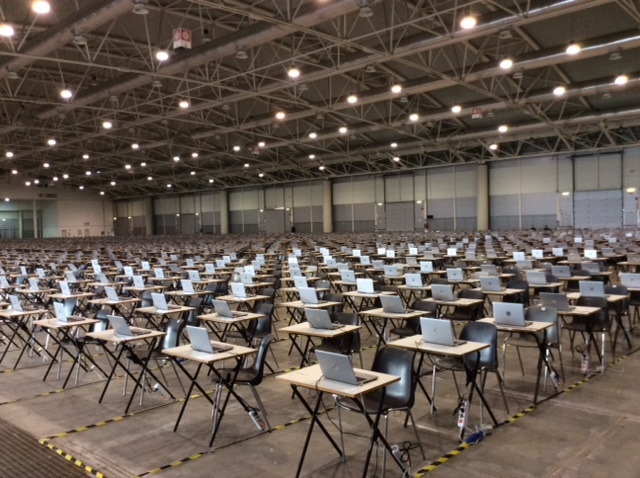
\includegraphics[width=0.40\textwidth]{figures/concorso-fiera-di-roma.jpg}
		\caption{Un concorso pubblico con elaborati digitali}
	\end{figure}
\end{frame}
\section{Specifica dei requisiti}
\begin{frame}
	\frametitle{Fase 2: Specifica dei requisiti}
	Partendo da questa idea lo step successivo è stata la definizione dei requisiti del progetto. Abbiamo perciò concordato che l’attività potesse orientarsi verso la creazione di un tool universale per la registrazione dell’impronta digitale (tramite funzioni di hashing) di insiemi di file, da noi battezzati Storage Unit, su Blockchain, utilizzando gli strumenti messi a disposizione da Git per gestirli meglio.
\end{frame}
\end{document}